\documentclass[
    11pt, % Set the default font size, options include: 8pt, 9pt, 10pt, 11pt, 12pt, 14pt, 17pt, 20pt
    aspectratio=169, % Set the aspect ratio to a 16:9 ratio which matches the aspect ratio of 1080p and 4K screens and projectors
]{beamer}

% This template is inspired by the VT Presentation Template, as well as the THU Beamer Theme. Many thanks!

\graphicspath{{images/}{./}} % Specifies where to look for included images (trailing slash required)
\usepackage{booktabs} % Allows the use of \toprule, \midrule and \bottomrule for better rules in tables
% \usepackage{appendixnumberbeamer} % If you want a separate slide counter for your appendix
\usepackage{fnpct} % Eliminate the unwanted space before the footnote mark
\usepackage{tikz} % Washed-out title background, pipeline diagram
\usetikzlibrary{arrows.meta, positioning}

\setbeamerfont{footnote}{size=\tiny}

%---------------------------------------------------------
%	SELECT THEME & COLORS
%---------------------------------------------------------
\usetheme{Madrid} % You can use other themes too, but this changes many things. I've found Madrid to be the best for this color scheme

% fg = foreground color
% bg = background color

% Many colors are linked to multiple attributes, change with caution!
\definecolor{fptBlue}{RGB}{0, 75, 145} % FPT blue (darkened for contrast)
\definecolor{fptOrange}{RGB}{243, 112, 33} % FPT orange

\setbeamercolor*{structure}{bg=fptBlue, fg=fptBlue}
% Title block and bottom right box color
\setbeamercolor*{palette primary}{use=structure, fg=white,bg=fptBlue} % Bottom left box and bar between title & top bubbles
\setbeamercolor*{palette secondary}{use=structure, fg=fptBlue, bg=white}
% Probably not used
\setbeamercolor*{palette tertiary}{use=structure, fg=white, bg=fptBlue} 

% Title of each slide
\setbeamercolor{frametitle}{bg=fptBlue, fg=white}
\setbeamercolor*{titlelike}{parent=palette primary}

%%% Headline and Central Footer %%%
% You can change the theme back and forth for each frame
% Theme I - white head, white foot
    % \setbeamercolor{section in head/foot}{fg=fptOrange, bg=white}
    % \setbeamercolor{headline}{fg=fptOrange, bg=white}
% Theme II - gold head, gold foot (as shown in the title frame)
    \setbeamercolor{section in head/foot}{fg=white, bg=fptOrange}
    \setbeamercolor{headline}{fg=white, bg=fptOrange}
% Theme III - white head, gold foot (as shown in the rest of the frames)
    % \setbeamercolor{section in head/foot}{fg=fptOrange, bg=white}
    % \setbeamercolor{title in head/foot}{fg=white, bg=fptOrange}
    % \setbeamercolor{headline}{fg=fptOrange, bg=white}

%%% Specific Colors %%%
\setbeamercolor{item projected}{bg=fptOrange}
\setbeamertemplate{enumerate items}{bg=fptOrange}

\setbeamercolor{itemize item}{fg=fptOrange}
\setbeamercolor{itemize subitem}{fg=fptOrange}

\setbeamercolor{button}{bg=fptOrange}

%%% Edits ONLY the TOC slide %%%
\setbeamercolor{section in toc}{fg=black}
\setbeamercolor{subsection in toc}{fg=black}

%%% Block Colors %%%
% Standard block
    \setbeamercolor{block title}{bg=fptOrange, fg=white}
    \setbeamercolor{block body}{bg=fptOrange!20}
% Alerted block
    \setbeamercolor{block title alerted}{bg=orange, fg=white}
    \setbeamercolor{block body alerted}{bg=orange!10}
% Example block
    \setbeamercolor{block title example}{bg=fptBlue, fg=white}
    \setbeamercolor{block body example}{bg=fptBlue!10}

%---------------------------------------------------------
%	SELECT THE FONT THEME & FONTS
%---------------------------------------------------------
\usefonttheme{default} % Typeset using the default sans serif font
\usepackage{palatino} % Use the Palatino font for serif text
\IfFileExists{opensans.sty}{\usepackage[default]{opensans}}{} % Open Sans for sans serif text, if installed
\useinnertheme{circles}

%---------------------------------------------------------
%	SELECT THE OUTER THEME
%---------------------------------------------------------
% Outer themes change the overall layout of slides, such as header and footer lines, sidebars and slide titles. Uncomment each theme in turns to see what changes it makes to your presentation.

% \useoutertheme{default}
\useoutertheme{miniframes}
% \useoutertheme{infolines}
% \useoutertheme{smoothbars}
% \useoutertheme{sidebar}
% \useoutertheme{split}
% \useoutertheme{shadow}
% \useoutertheme{tree}
% \useoutertheme{smoothtree}

%---------------------------------------------------------
%	PRESENTATION INFORMATION
%---------------------------------------------------------
\title[NightClear]{NightClear: Robust Low-Light Image Restoration}
% Click the middle footer can switch between the first and last numbered frame
\subtitle{Joint low-light enhancement and deblurring for night photography}
\author[Duc, Truong, Tuan]{\texorpdfstring{%
    \begin{tabular}{ll}
        Mai Xuan Duc & SE196257 \\
        Phan Minh Nhat Truong & SE196744 \\
        Dang Thanh Tuan & SE196418
    \end{tabular}}{Mai Xuan Duc, Phan Minh Nhat Truong, Dang Thanh Tuan}}

\institute[FPTU]{Supervisor: Mr. Nguyen Trong Tai \quad$\cdot$\quad FPT University}
\date[15/11/2026]{November 15, 2026}

% School logo: shown at the top-right of the headline; \logo{} hides it for a frame
\newcommand{\fptlogo}{
\includegraphics[height=0.6cm]{Logo_FPT_Education.png}}
\logo{\fptlogo}


%---------------------------------------------------------
%	EXTRA SETTINGS
%---------------------------------------------------------

% Clear warnings related to \translate
%     https://github.com/josephwright/beamer/issues/449
\pdfstringdefDisableCommands{
    \def\translate#1{#1}
}

% Simple header: logo on the left, current section name on the right (plain text, no links)
% Section name in the header: larger and bold so it reads on a projector
\setbeamerfont{section in head/foot}{size=\small, series=\bfseries}
\setbeamertemplate{headline}{%
    \nointerlineskip
    \begin{beamercolorbox}[wd=\paperwidth,ht=1cm,dp=0pt]{headline}%
        % both boxes are vertically centred in the 1cm header so the logo never touches the title bar
        \raisebox{0.5cm}{\parbox[c]{0.5\paperwidth}{\hspace*{2mm}\insertlogo}}%
        \hfill\raisebox{0.5cm}{\parbox[c]{0.48\paperwidth}{\raggedleft\usebeamerfont{section in head/foot}\insertsectionhead\hspace*{4mm}}}%
    \end{beamercolorbox}%
}
% Logo lives in the headline, not the bottom-right corner
\setbeamertemplate{sidebar right}{}

% Footer: two equal halves, plain text (no author box, no links)
\setbeamertemplate{footline}{%
    \leavevmode%
    \hbox{%
        \begin{beamercolorbox}[wd=.5\paperwidth, ht=2.5ex, dp=1ex, center]{title in head/foot}%
            \usebeamerfont{title in head/foot}\inserttitle
        \end{beamercolorbox}%
        \begin{beamercolorbox}[wd=.5\paperwidth, ht=2.5ex, dp=1ex, center]{date in head/foot}%
            \usebeamerfont{date in head/foot}FPT University \quad$\cdot$\quad \insertshortdate \quad$\cdot$\quad \insertframenumber{} / \inserttotalframenumber
        \end{beamercolorbox}}%
    \vskip0pt%
}

% Disable navigation symbols
\setbeamertemplate{navigation symbols}{}

%---------------------------------------------------------
%   DOCUMENT BEGINS
%---------------------------------------------------------
\begin{document}

%---------------------------------------------------------
%	TITLE SLIDE
%---------------------------------------------------------
\section{}

% Set background
\usebackgroundtemplate{%
    \begin{tikzpicture}
        \clip (0,0) rectangle (\paperwidth,\paperheight); % crop the 3:2 photo to 16:9 without stretching
        \node[inner sep=0, opacity=0.25] at ({0.5\paperwidth},{0.5\paperheight}) {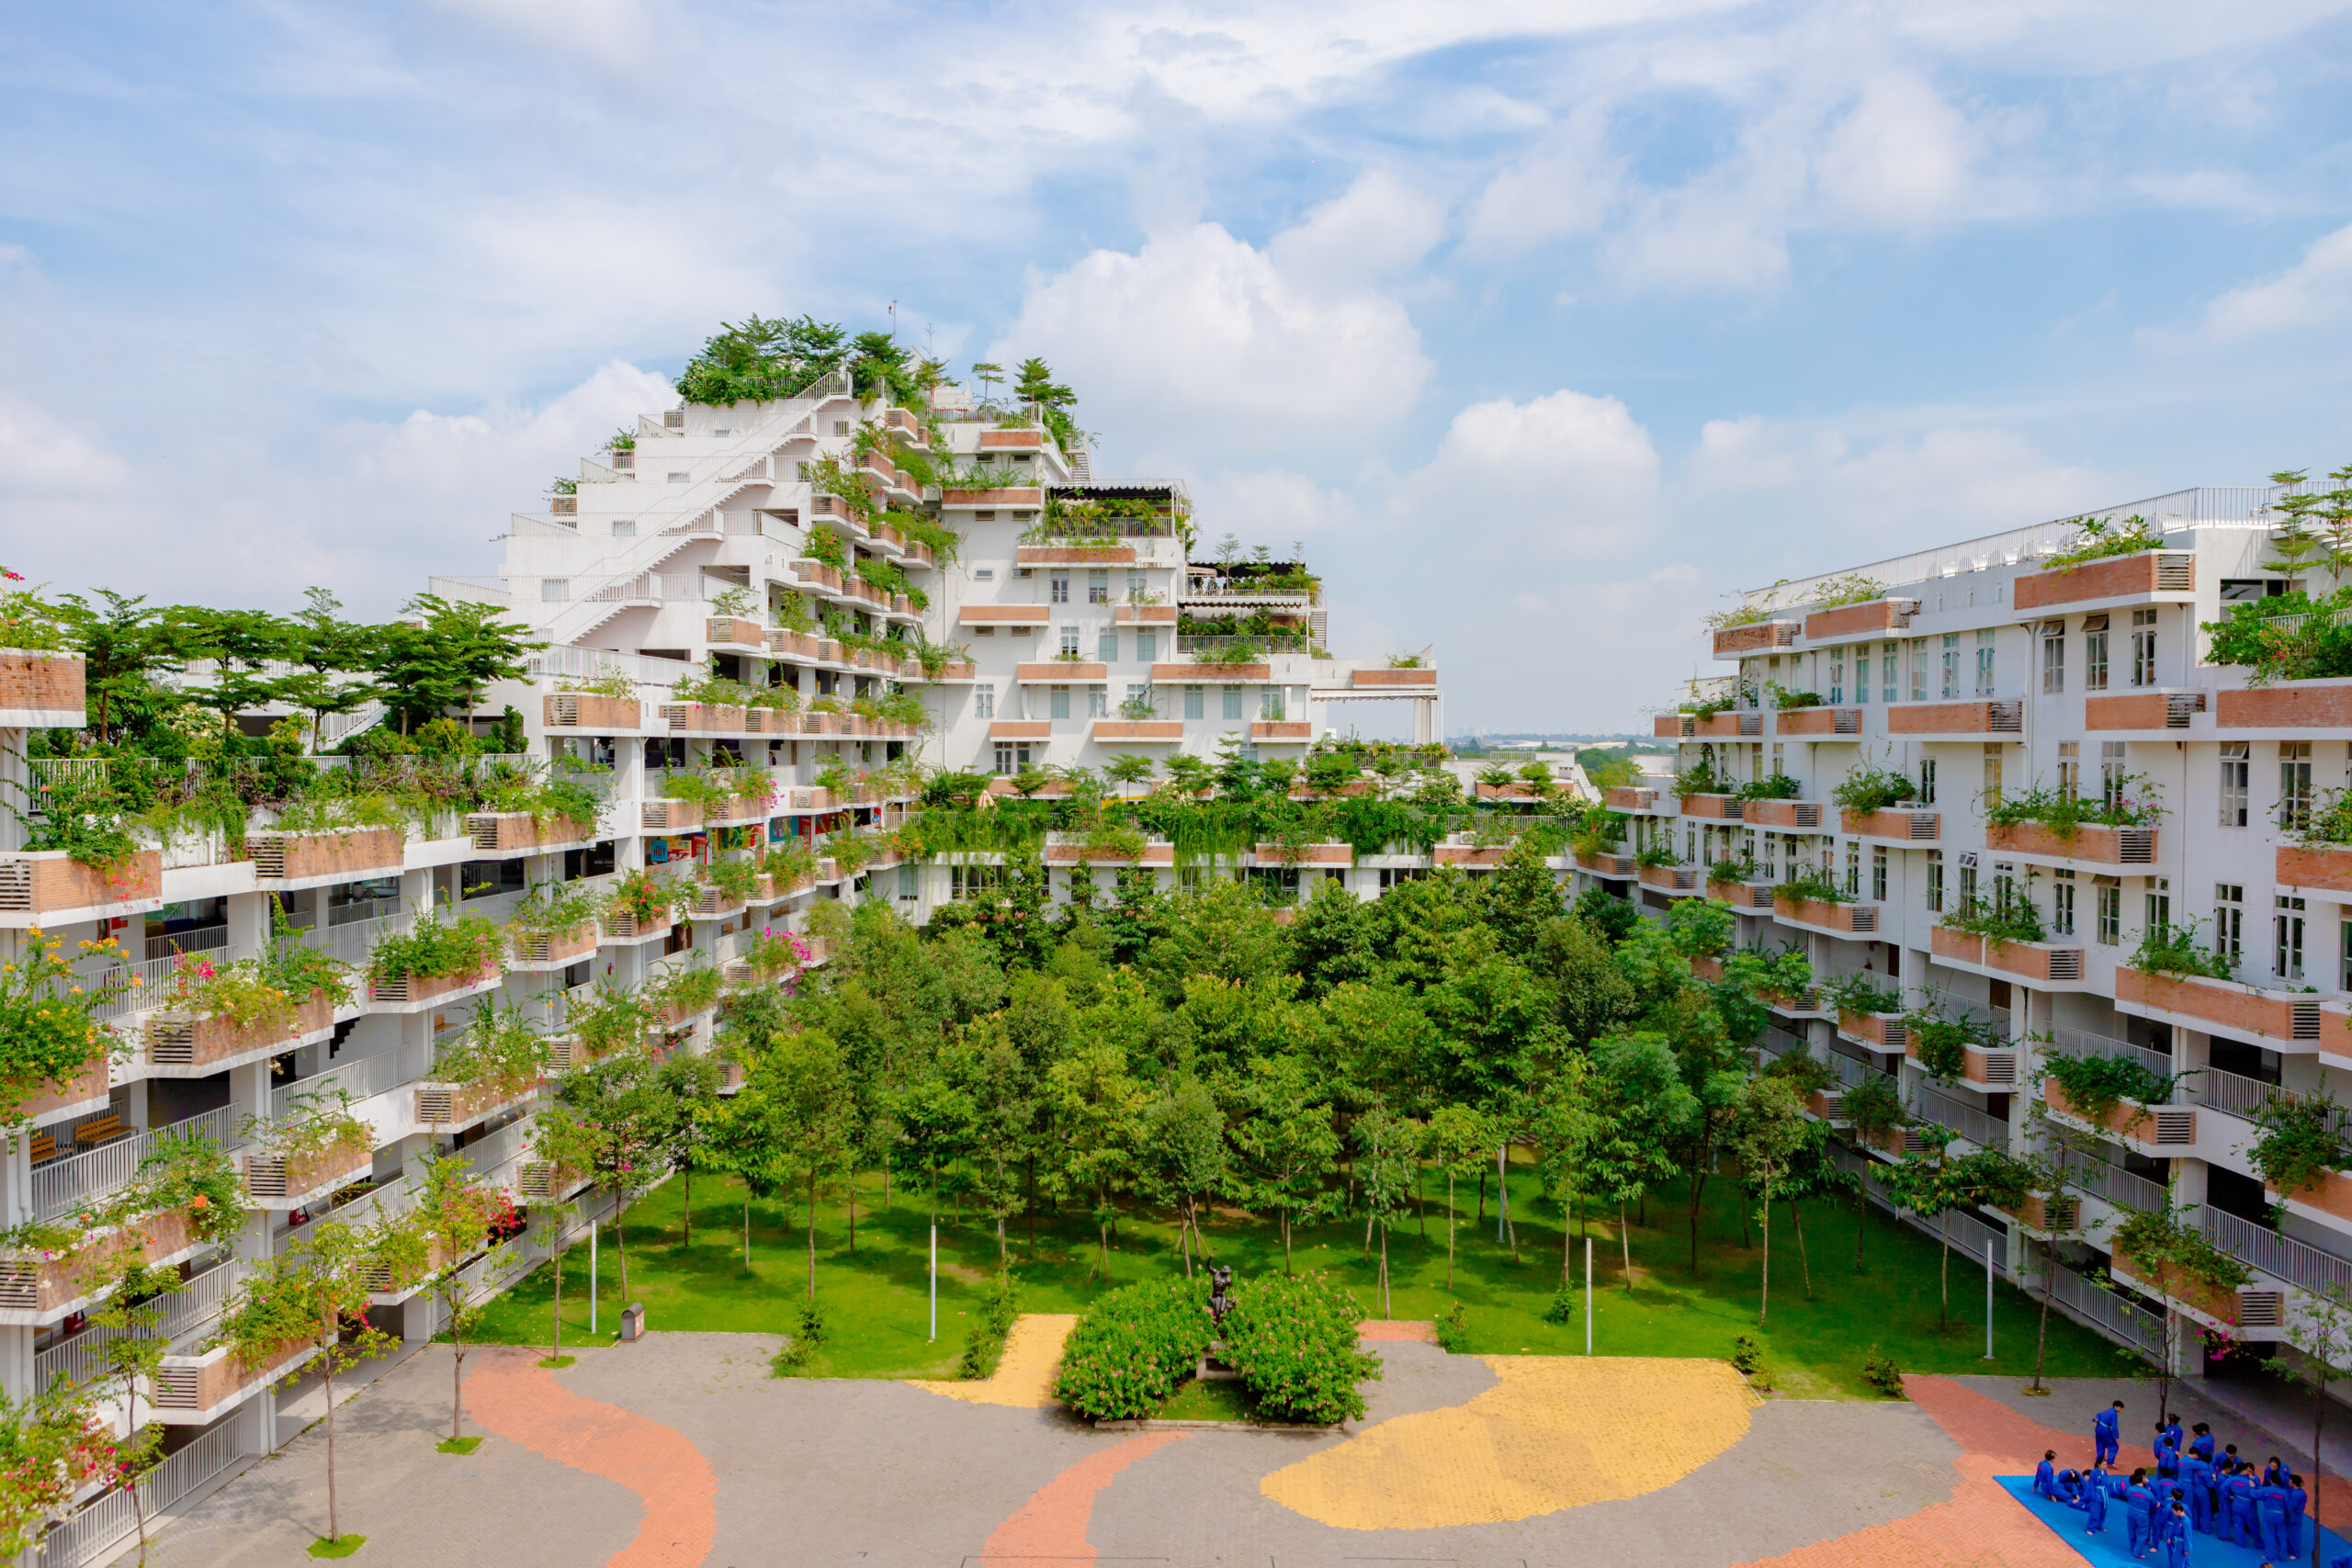
\includegraphics[width=\paperwidth]{P.Zo-9862-scaled-1.jpg}};
        % FPT logo top-left, just below the headline and above the title box
        \node[anchor=north west, inner sep=0] at (4mm,{\paperheight-0.9cm}) {
\includegraphics[height=0.85cm]{Logo_FPT_Education.png}};
    \end{tikzpicture}%
}
% Disable logo
\logo{}

\begin{frame}
	\titlepage % Output the title slide, automatically created using the text entered in the PRESENTATION INFORMATION block above
\end{frame}

% Clear background
\usebackgroundtemplate{}
% Enable logo
\logo{\fptlogo}

% Switch to Theme III
\setbeamercolor{section in head/foot}{fg=fptOrange, bg=white}
\setbeamercolor{title in head/foot}{fg=white, bg=fptOrange}
\setbeamercolor{headline}{fg=fptOrange, bg=white}

%---------------------------------------------------------
%	TABLE OF CONTENTS SLIDE
%	Two balanced columns, 3 sections each. Section 1 is the empty title-slide section.
%---------------------------------------------------------
{% local: more air between entries, only on this slide
\addtobeamertemplate{section in toc}{\vspace{5mm}}{}
\begin{frame}
    \frametitle{Table of Contents}
    \vfill
    \centering
    \begin{minipage}[t]{0.3\textwidth}
        \Large
        \tableofcontents[sections={2-4}]
    \end{minipage}%
    \hspace{0.08\textwidth}%
    \begin{minipage}[t]{0.3\textwidth}
        \Large
        \tableofcontents[sections={5-7}]
    \end{minipage}
    \vfill
\end{frame}
}

%---------------------------------------------------------
%	2. PROBLEM STATEMENT & OBJECTIVES
%---------------------------------------------------------
\section{Problem}

\begin{frame}
    \frametitle{Problem Statement}
    \framesubtitle{Night photography degrades images in three ways at once}

    \begin{columns}[c]
        \begin{column}{0.52\textwidth}
            \small
            Small phone sensors + fixed aperture $\Rightarrow$ \textbf{long exposures} at night:
            \begin{itemize}
                \item \textbf{Low light}: dark, low-contrast images
                \item \textbf{Noise}: shot / read noise of the sensor
                \item \textbf{Motion blur}: hand shake during the exposure
            \end{itemize}
            Image formation model:
            \[
                y = \gamma\big(x \otimes k\big) + n
            \]
            {\footnotesize $y$: captured image, $x$: clean scene, $k$: blur kernel, $n$: noise, $\gamma$: dynamic-range loss}

            \textbf{Goal:} recover $x$ from a single $y$ --- brighten, denoise \emph{and} deblur in one model.
        \end{column}
        \begin{column}{0.46\textwidth}
            \centering
            \includegraphics[height=0.31\textheight]{../../assets/teaser/0085_low.png}\\[-0.5mm]
            {\scriptsize Input: low light + blur + noise}\\[1.5mm]
            \includegraphics[height=0.31\textheight]{../../assets/teaser/0085_darkir.png}\\[-0.5mm]
            {\scriptsize NightClear output}
        \end{column}
    \end{columns}
\end{frame}

\begin{frame}
    \frametitle{Why Data Science? Objectives \& KPIs}

    \begin{columns}[t]
        \begin{column}{0.47\textwidth}
            \small
            \textbf{Why a data-driven model}
            \begin{itemize}
                \item The needed brightening is image-dependent: \textbf{$\times$2.8 to $\times$30} across LOLv2-real pairs (our EDA) --- no fixed curve fits all.
                \item Chaining two specialised models fails: \textbf{14.7--18.3\,dB} vs.\ \textbf{27.0\,dB} for one joint model.
                \item 10k+ paired examples (LOL-Blur) let a network learn the inverse mapping directly.
            \end{itemize}
        \end{column}
        \begin{column}{0.51\textwidth}
            \small
            \textbf{KPIs} {\footnotesize (target = beat LEDNet, the previous joint method)}\\[1mm]
            \footnotesize
            \begin{tabular}{lll}
                \toprule
                \textbf{Metric (LOLBlur)} & \textbf{Target} & \textbf{NightClear-m} \\
                \midrule
                PSNR $\uparrow$  & $> 25.74$ dB & \textbf{27.00} $\checkmark$ \\
                SSIM $\uparrow$  & $> 0.850$    & \textbf{0.883} $\checkmark$ \\
                LPIPS $\downarrow$ & $< 0.224$  & \textbf{0.162} $\checkmark$ \\
                Compute          & $< 10$ GMACs & \textbf{7.25} $\checkmark$ \\
                Model size       & $< 5$ M params & \textbf{3.31} $\checkmark$ \\
                Deployment       & usable app   & Gradio UI $\checkmark$ \\
                \bottomrule
            \end{tabular}
        \end{column}
    \end{columns}
\end{frame}

%---------------------------------------------------------
%	3.1 - 3.2 DATA (sizes from the DarkIR README / paper, EDA from presentation/eda/eda_lolv2.py)
%---------------------------------------------------------
\section{Data}

\begin{frame}
    \frametitle{Dataset Overview}
    \framesubtitle{Each sample = a (low-light, ground-truth) pair of RGB images}

    \begin{center}
    \scriptsize
    \begin{tabular}{llrrll}
        \toprule
        \textbf{Dataset} & \textbf{Degradation} & \textbf{Train} & \textbf{Test} & \textbf{Resolution} & \textbf{Source} \\
        \midrule
        LOL-Blur     & low light + blur + noise & 10{,}200 & 1{,}800 & 1120$\times$640 & LEDNet \\
        LOLv2-real   & low light        & 689      & 100     & 600$\times$400 & LOLv2 \\
        LOLv2-synth  & low light        & 900      & 100     & 384$\times$384 & LOLv2 \\
        LSRW (Nikon / Huawei) & low light & 5{,}600 & 50   & varies & R2RNet \\
        \midrule
        Real-LOLBlur, DICM, LIME, MEF, NPE, VV & real night photos & \multicolumn{2}{c}{unpaired, test only} & varies & -- \\
        \bottomrule
    \end{tabular}
    \end{center}

    \begin{columns}[t]
        \begin{column}{0.5\textwidth}
            \footnotesize
            \textbf{Raw-data issues}
            \begin{itemize}
                \item No missing / corrupt files; every input has its GT (checked on LOLv2)
                \item \textbf{Imbalance}: LOL-Blur is 57\% of all paired training data
                \item Tiny test sets (LSRW 20--30 pairs) $\Rightarrow$ noisy scores
            \end{itemize}
        \end{column}
        \begin{column}{0.5\textwidth}
            \footnotesize
            \textbf{Preprocessing}
            \begin{itemize}
                \item Train: random 384$\times$384 crops, flips and rotations
                \item Pixels scaled to $[0, 1]$; pad to a multiple of 8 (3 down-sampling stages)
                \item Deploy: optional resize (max side 1280\,px)
            \end{itemize}
        \end{column}
    \end{columns}
\end{frame}

\begin{frame}
    \frametitle{Key EDA Insights (1/2): How Dark Is the Data?}
    \framesubtitle{LOLv2 real + synthetic, all 1{,}789 pairs, luminance $Y \in [0, 1]$}

    \begin{center}
        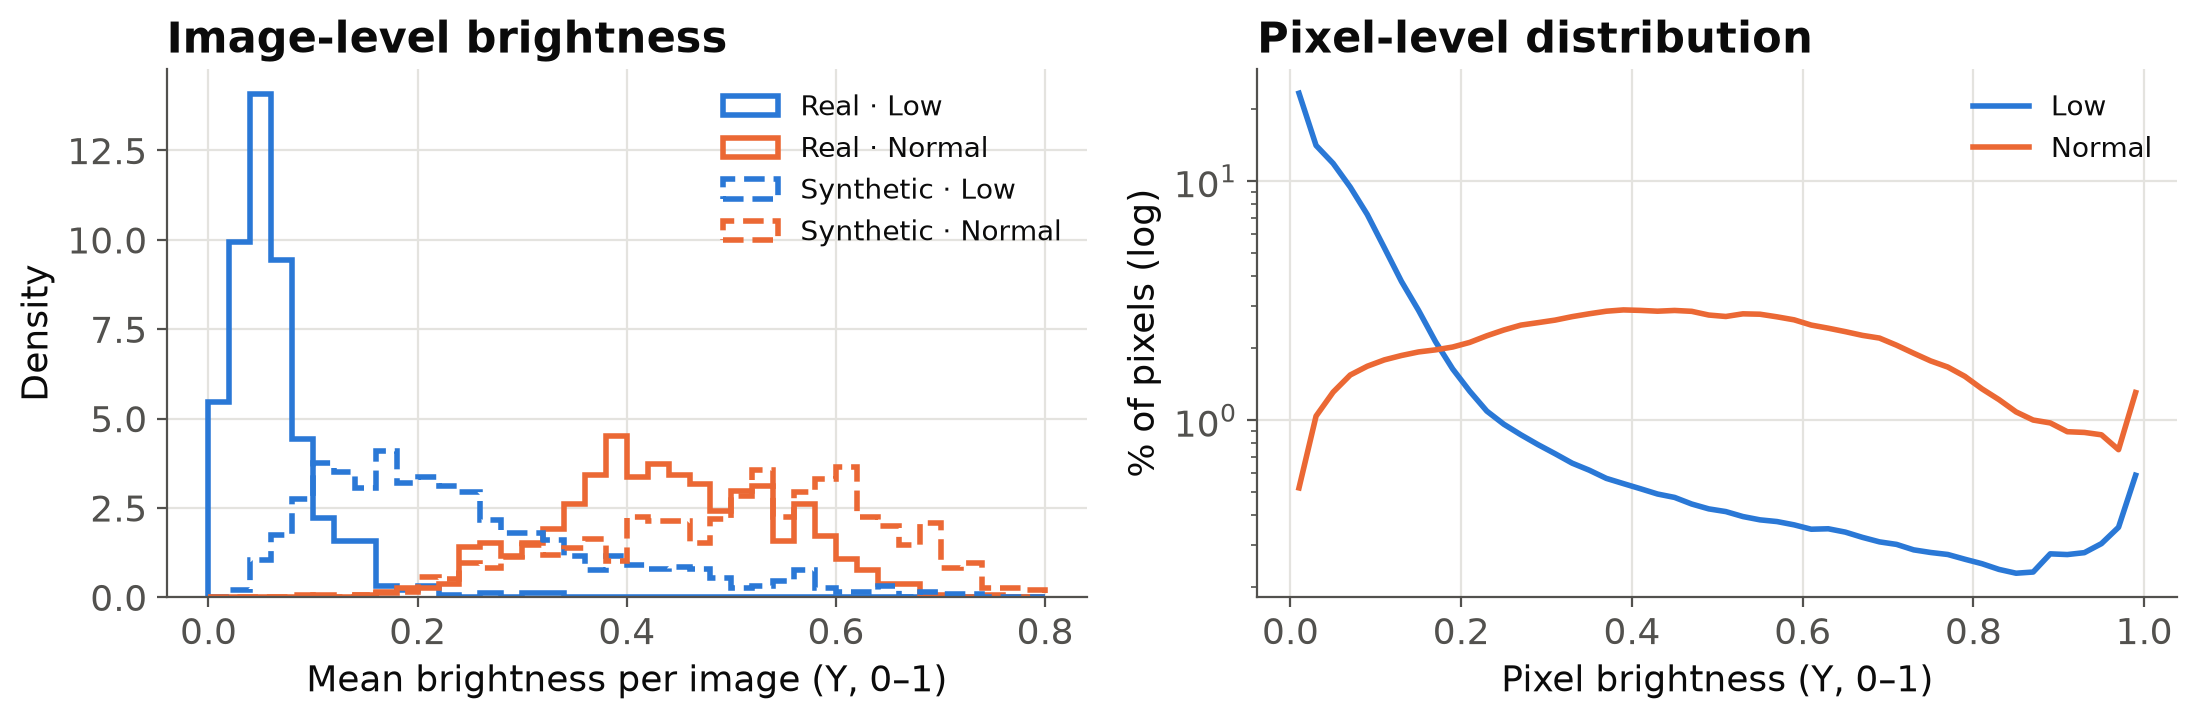
\includegraphics[width=\textwidth, height=0.52\textheight, keepaspectratio]{eda/brightness.png}
    \end{center}
    \vspace{-2mm}
    \begin{columns}[t]
        \begin{column}{0.5\textwidth}
            \footnotesize
            \textbf{Left:} real low-light images average $Y = 0.06$ vs.\ $0.44$ for GT; synthetic ones are much brighter ($0.24$) $\Rightarrow$ \textbf{real/synthetic domain gap}.
        \end{column}
        \begin{column}{0.5\textwidth}
            \footnotesize
            \textbf{Right:} 81\% of real low-light pixels have $Y < 0.1$ $\Rightarrow$ most information sits in a few dark grey levels, where noise dominates.
        \end{column}
    \end{columns}
\end{frame}

\begin{frame}
    \frametitle{Key EDA Insights (2/2): Brightening Is Not One Curve}
    \begin{columns}[c]
        \begin{column}{0.5\textwidth}
            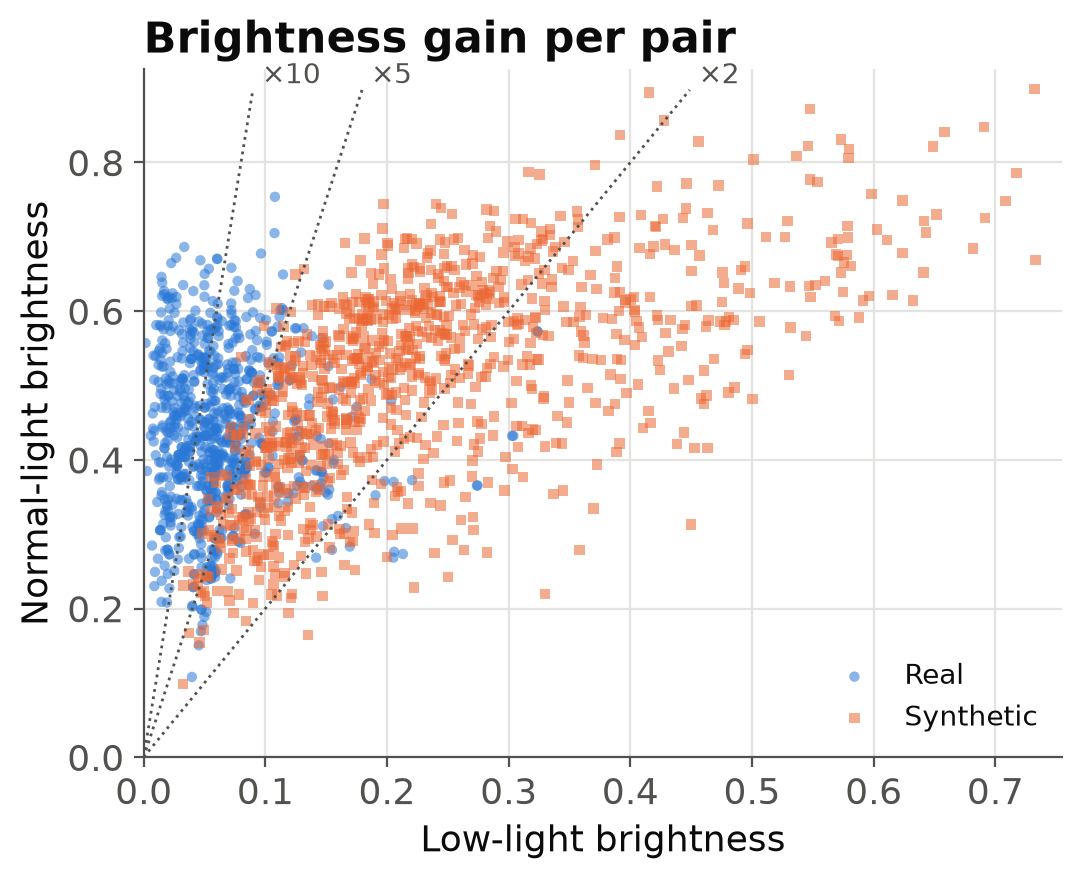
\includegraphics[width=\textwidth]{eda/gain_scatter.png}
        \end{column}
        \begin{column}{0.48\textwidth}
            \small
            Gain = GT brightness / low-light brightness
            \begin{itemize}
                \item Real: median $\times 7.5$, 90\% of pairs between $\times 2.8$ and $\times 30$.
                \item Synthetic: median $\times 2.5$ ($\times 1.1$ -- $\times 4.8$).
            \end{itemize}
            \vspace{2mm}
            \textbf{Conclusion:} the required brightening changes from image to image, so a global curve (gamma, histogram equalisation) cannot fit all pairs $\Rightarrow$ the model must learn \emph{content-aware} enhancement.
        \end{column}
    \end{columns}
\end{frame}

%---------------------------------------------------------
%	3.3 METHODOLOGY & ARCHITECTURE
%---------------------------------------------------------
\section{Method}

\begin{frame}
    \frametitle{Solution Pipeline}
    \framesubtitle{From raw night photos to a deployed restoration service}

    \begin{center}
    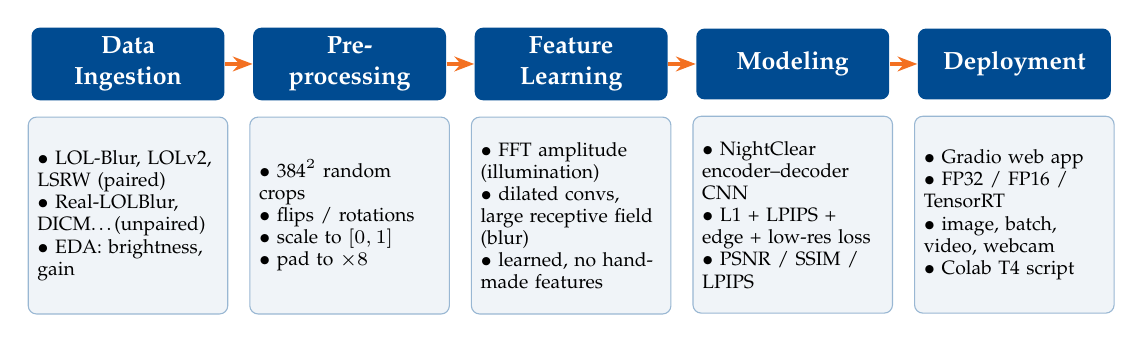
\begin{tikzpicture}[
        stage/.style={rectangle, rounded corners=3pt, fill=fptBlue, text=white, font=\small\bfseries,
                      minimum width=2.45cm, minimum height=0.9cm, align=center},
        detail/.style={rectangle, rounded corners=3pt, draw=fptBlue!40, fill=fptBlue!6, font=\scriptsize,
                       text width=2.3cm, minimum height=2.5cm, align=left, anchor=north},
        arrow/.style={-{Stealth[length=2.5mm]}, very thick, fptOrange},
        node distance=0.35cm]
        \node[stage] (s1) {Data\\Ingestion};
        \node[stage, right=of s1] (s2) {Pre-\\processing};
        \node[stage, right=of s2] (s3) {Feature\\Learning};
        \node[stage, right=of s3] (s4) {Modeling};
        \node[stage, right=of s4] (s5) {Deployment};
        \foreach \a/\b in {s1/s2, s2/s3, s3/s4, s4/s5} \draw[arrow] (\a) -- (\b);

        \node[detail] at ([yshift=-2mm]s1.south) {
            $\bullet$ LOL-Blur, LOLv2, LSRW (paired)\\
            $\bullet$ Real-LOLBlur, DICM\ldots (unpaired)\\
            $\bullet$ EDA: brightness, gain};
        \node[detail] at ([yshift=-2mm]s2.south) {
            $\bullet$ 384$^2$ random crops\\
            $\bullet$ flips / rotations\\
            $\bullet$ scale to $[0,1]$\\
            $\bullet$ pad to $\times 8$};
        \node[detail] at ([yshift=-2mm]s3.south) {
            $\bullet$ FFT amplitude (illumination)\\
            $\bullet$ dilated convs, large receptive field (blur)\\
            $\bullet$ learned, no hand-made features};
        \node[detail] at ([yshift=-2mm]s4.south) {
            $\bullet$ NightClear encoder--decoder CNN\\
            $\bullet$ L1 + LPIPS + edge + low-res loss\\
            $\bullet$ PSNR / SSIM / LPIPS};
        \node[detail] at ([yshift=-2mm]s5.south) {
            $\bullet$ Gradio web app\\
            $\bullet$ FP32 / FP16 / TensorRT\\
            $\bullet$ image, batch, video, webcam\\
            $\bullet$ Colab T4 script};
    \end{tikzpicture}
    \end{center}
\end{frame}

\begin{frame}
    \frametitle{NightClear Architecture \& Training}

    \begin{center}
        \includegraphics[height=0.37\textheight]{../../assets/networks-scheme.png}
    \end{center}
    \vspace{-1mm}
    \begin{columns}[t]
        \begin{column}{0.5\textwidth}
            \footnotesize
            \textbf{Encoder = illumination (Fourier domain)}
            \begin{itemize}
                \item EBlock: attention + \textbf{FreMLP} (MLP on the FFT \emph{amplitude})
                \item Bottleneck predicts an 8$\times$ smaller lit image
            \end{itemize}
            \textbf{Decoder = deblurring (spatial domain)}
            \begin{itemize}
                \item DBlock: \textbf{Di-SpAM}, dilated depthwise convs (1, 4, 9)
            \end{itemize}
        \end{column}
        \begin{column}{0.5\textwidth}
            \footnotesize
            \textbf{Training}
            \begin{itemize}
                \item Loss: $\mathcal{L} = \mathcal{L}_{1} + 0.01\,\mathcal{L}_{\text{LPIPS}} + 50\,\mathcal{L}_{\text{edge}} + \mathcal{L}_{\text{low-res}}$
                \item AdamW, LR $5\!\times\!10^{-4} \rightarrow 10^{-6}$ cosine, batch 32, H100
                \item NightClear-m: width 32, \textbf{3.31 M params, 7.25 GMACs}
            \end{itemize}
        \end{column}
    \end{columns}
\end{frame}

%---------------------------------------------------------
%	4. MODELING & EVALUATION (numbers: DarkIR paper, arXiv 2412.13443)
%---------------------------------------------------------
\section{Results}

\begin{frame}
    \frametitle{Model Experimentation}
    \framesubtitle{Baselines vs.\ advanced models on LOLBlur}

    \begin{columns}[t]
        \begin{column}{0.56\textwidth}
            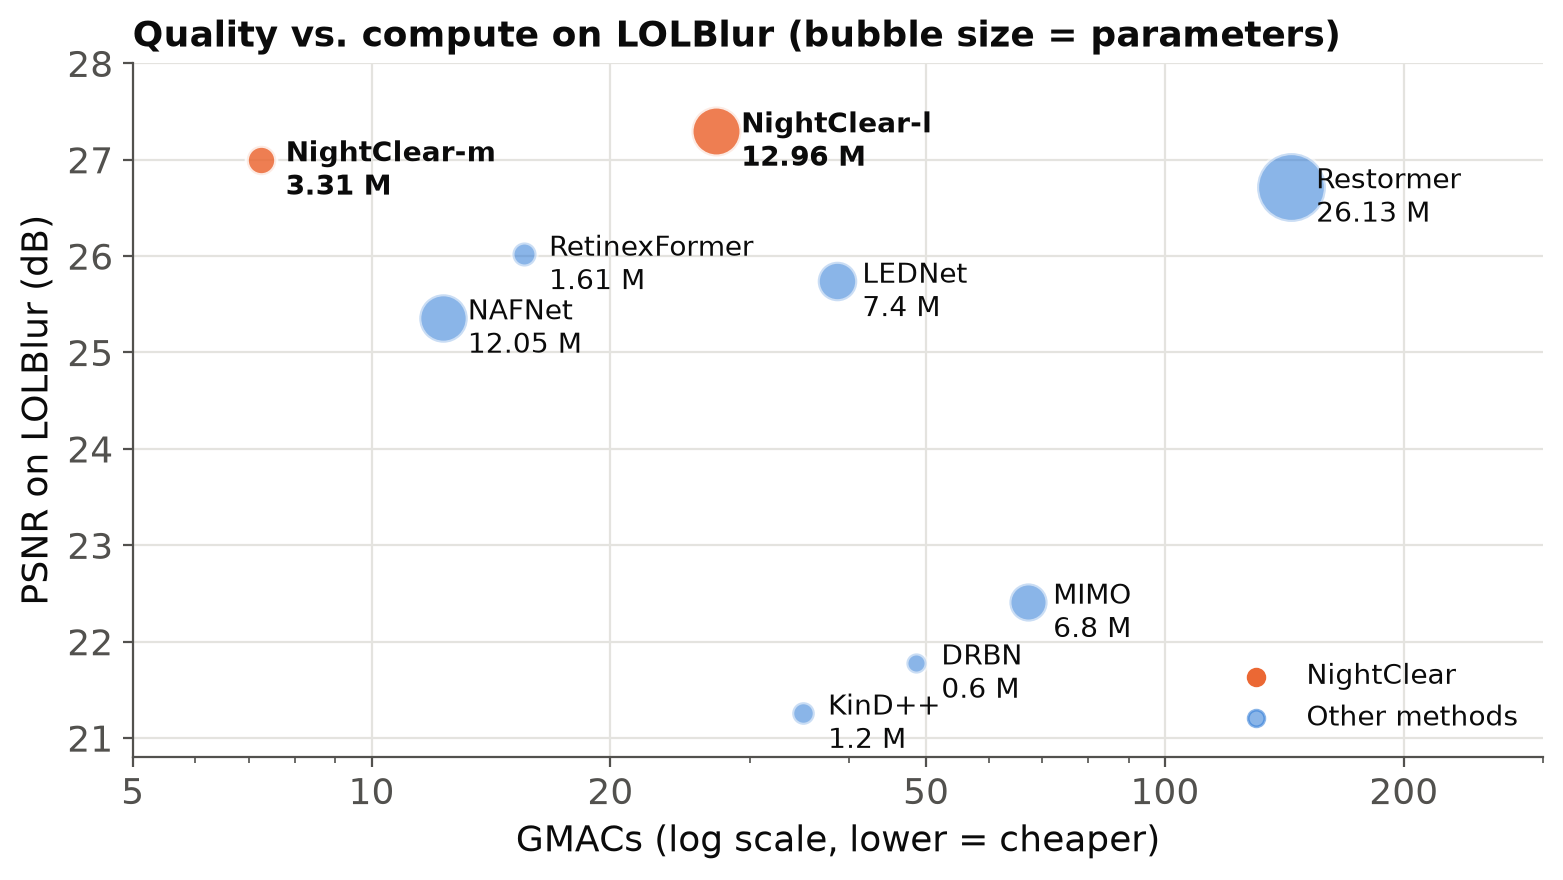
\includegraphics[width=\textwidth, height=0.55\textheight, keepaspectratio]{results/efficiency.png}\\
            \footnotesize NightClear-m reaches the best PSNR with the \textbf{lowest compute} (7.25 GMACs, 20$\times$ less than Restormer).
        \end{column}
        \begin{column}{0.42\textwidth}
            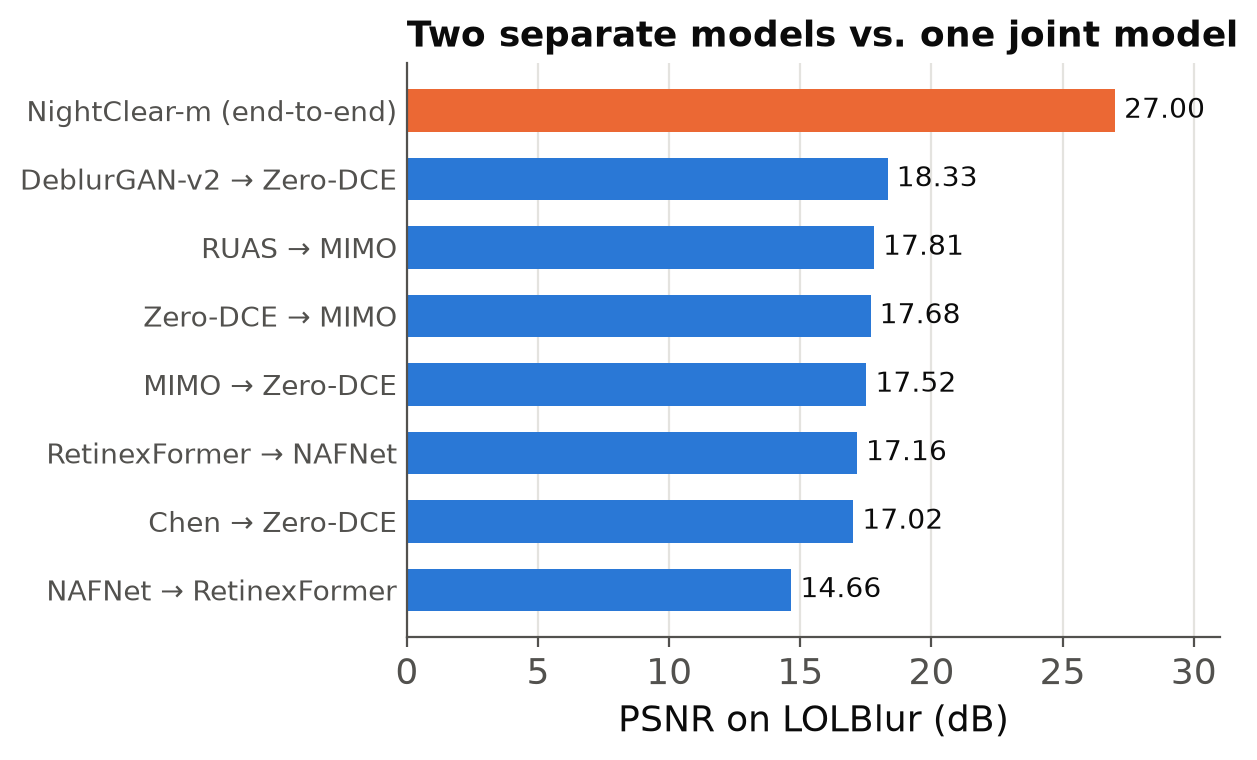
\includegraphics[width=\textwidth, height=0.55\textheight, keepaspectratio]{results/cascade.png}\\
            \footnotesize Every two-model cascade stays below 18.4\,dB; one joint model gains \textbf{+8.7\,dB}.
        \end{column}
    \end{columns}
    \vspace{1mm}
    {\tiny DeblurGAN-v2 (22.30 dB) is not plotted: no MACs available.}
\end{frame}

\begin{frame}
    \frametitle{Evaluation Across Datasets}
    \framesubtitle{Best other method per row; bold = better value}

    \begin{center}
    \footnotesize
    \begin{tabular}{lllll}
        \toprule
        \textbf{Dataset} & \textbf{Metric} & \textbf{NightClear} & \textbf{Best other method} & \\
        \midrule
        LOLBlur & PSNR $\uparrow$  & \textbf{27.00} (m) / \textbf{27.30} (l) & 26.72 & Restormer \\
                & SSIM $\uparrow$  & 0.883 / 0.898 & \textbf{0.902} & Restormer \\
                & LPIPS $\downarrow$ & 0.162 / 0.137 & \textbf{0.133} & Restormer \\
        LOLv2-real  & PSNR / SSIM & \textbf{23.87} / \textbf{0.880} & 22.80 / 0.840 & Retinexformer \\
        LOLv2-synth & PSNR / SSIM & 25.54 / \textbf{0.934} & \textbf{25.67} / 0.930 & Retinexformer \\
        LSRW        & PSNR / SSIM & \textbf{18.93} / \textbf{0.583} & 17.67 / 0.549 & FIDE \\
        Real-LOLBlur & MUSIQ $\uparrow$ / NIQE $\downarrow$ & 48.36 / 4.998 & \textbf{50.22} / \textbf{4.576} & NAFNet / Retinexformer \\
        \bottomrule
    \end{tabular}
    \end{center}
    \vspace{1mm}
    \footnotesize
    \begin{itemize}
        \item Best PSNR on 3 of the 4 paired benchmarks, with 8$\times$ fewer parameters than Restormer.
        \item Not the best everywhere: Restormer has better SSIM / LPIPS on LOLBlur, and on real blurry night photos (no GT) NightClear is competitive but not first.
    \end{itemize}
    {\tiny LOLv2 / LSRW use NightClear-mt (multi-task model, 26.62 dB on LOLBlur).}
\end{frame}

\begin{frame}
    \frametitle{Error Analysis}
    \framesubtitle{Released outputs on LOLv2-real image 00733: where does each model fail?}

    \begin{center}
        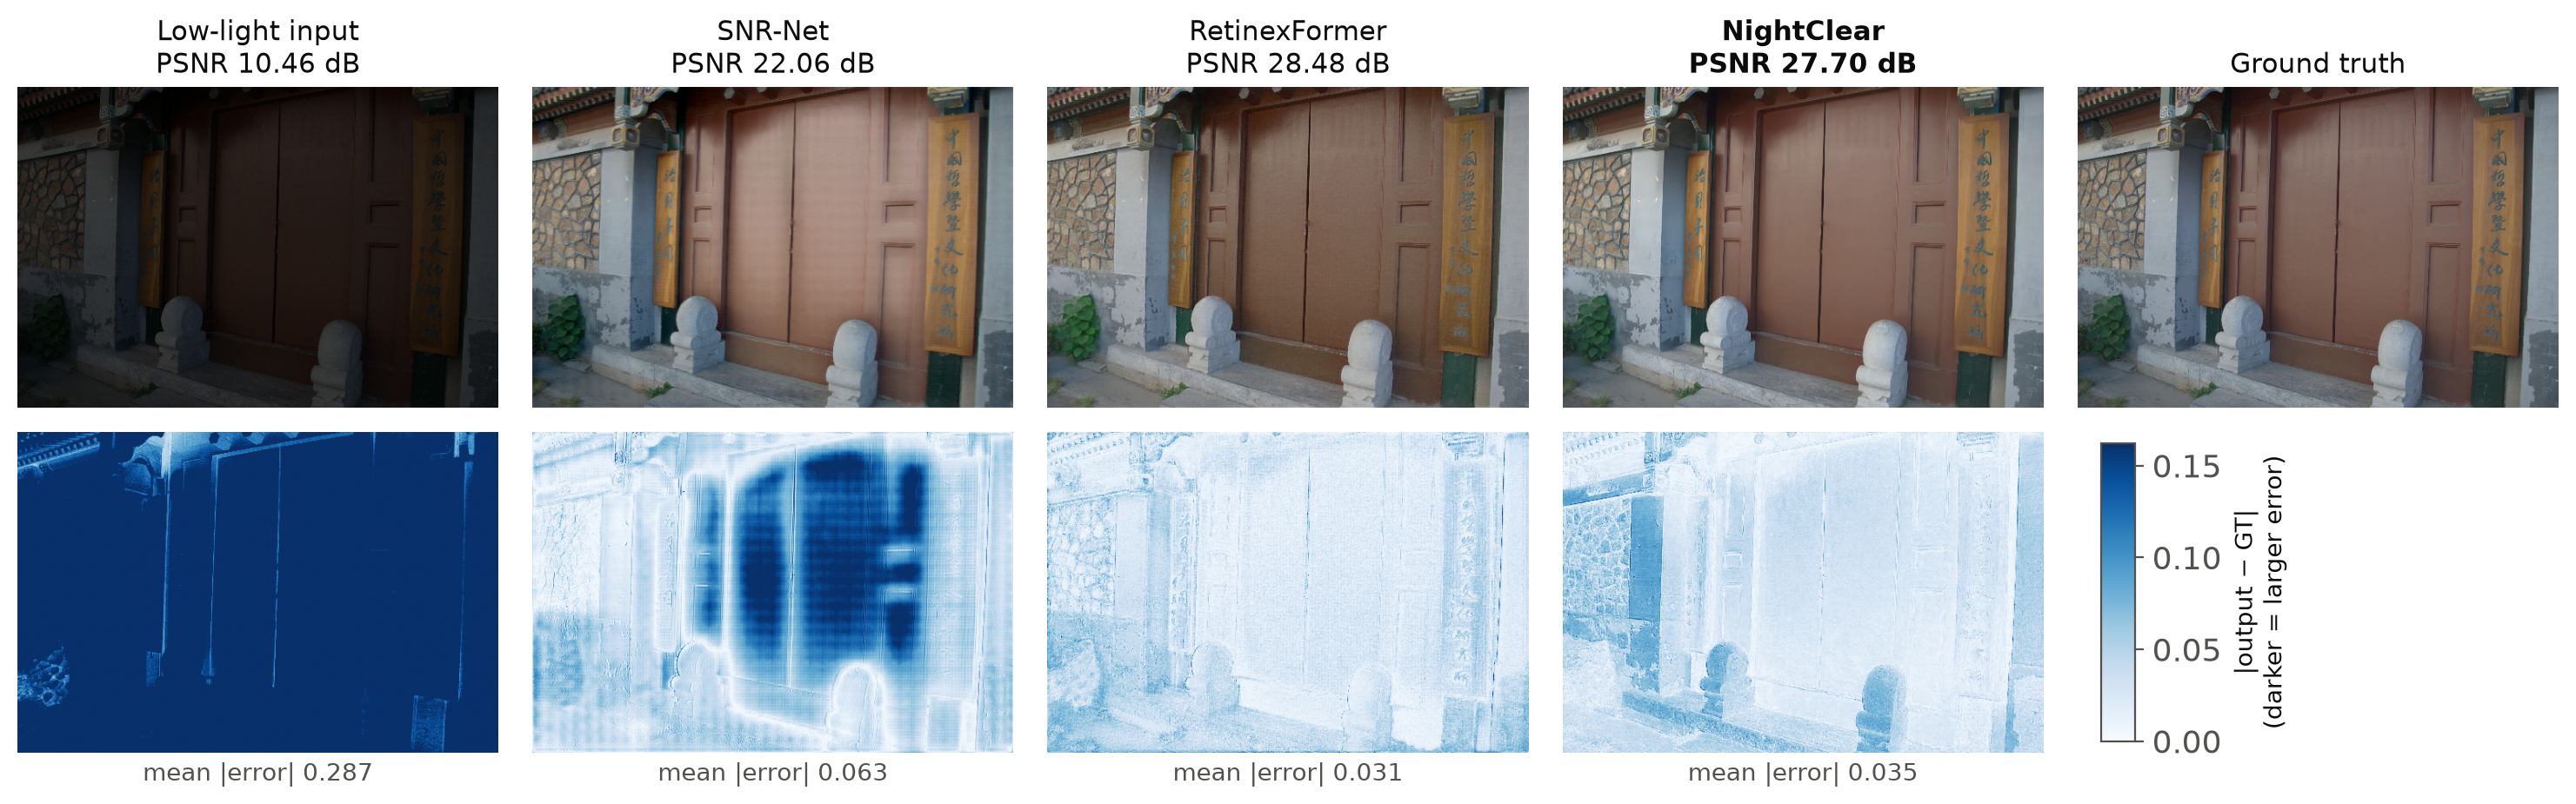
\includegraphics[width=\textwidth, height=0.46\textheight, keepaspectratio]{results/error_maps.png}
    \end{center}
    \footnotesize
    \begin{itemize}
        \item On this image Retinexformer (28.48\,dB) beats NightClear (27.70\,dB): NightClear's errors sit on the \textbf{textured stone wall and dark shadows} (tone shift).
        \item SNR-Net leaves blotchy artefacts on the large flat door.
        \item Takeaway: what remains is mostly \textbf{tone error in dark, textured regions}, consistent with the EDA (very dark pixels carry little signal).
    \end{itemize}
\end{frame}

%---------------------------------------------------------
%	5. MODEL INTERPRETABILITY
%	SHAP / feature importance do not fit an image-to-image model; component ablation plays that role.
%---------------------------------------------------------
\begin{frame}
    \frametitle{Model Interpretability (1/2): Which Components Matter?}
    \framesubtitle{Component importance = PSNR lost when a part is removed or replaced (paper ablations)}

    \begin{center}
        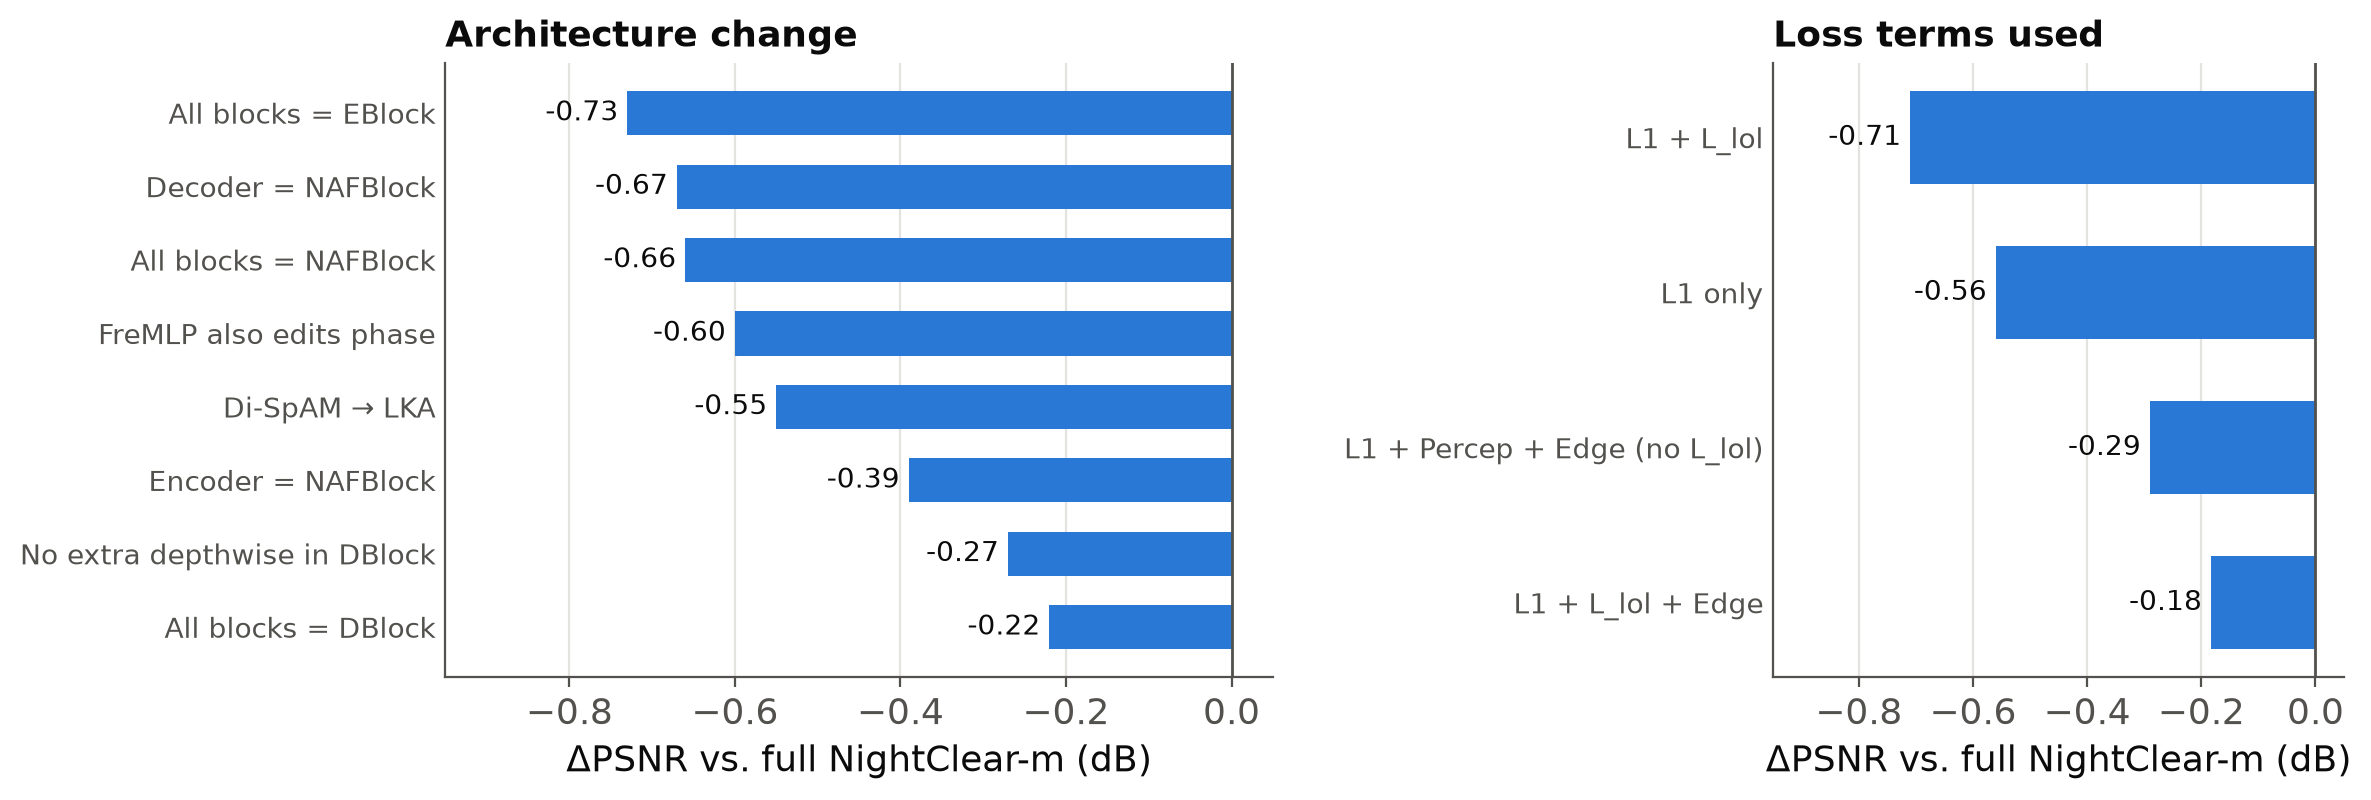
\includegraphics[width=\textwidth, height=0.47\textheight, keepaspectratio]{results/ablation.png}
    \end{center}
    \footnotesize
    \begin{itemize}
        \item Using the \textbf{same block everywhere} costs up to 0.73\,dB: the encoder (illumination) and the decoder (deblurring) need different designs.
        \item The low-res supervision $\mathcal{L}_{\text{low-res}}$ only helps together with the perceptual and edge losses (all four terms give the best PSNR).
    \end{itemize}
    {\tiny Table 6 and A: 256\,px training crops, full model 26.90\,dB; Table 7: full model 27.00\,dB.}
\end{frame}

\begin{frame}
    \frametitle{Model Interpretability (2/2): Why the Fourier Amplitude?}
    \framesubtitle{Our experiment on the 100 LOLv2-real test pairs: swap the FFT amplitude, keep the phase}

    \begin{center}
        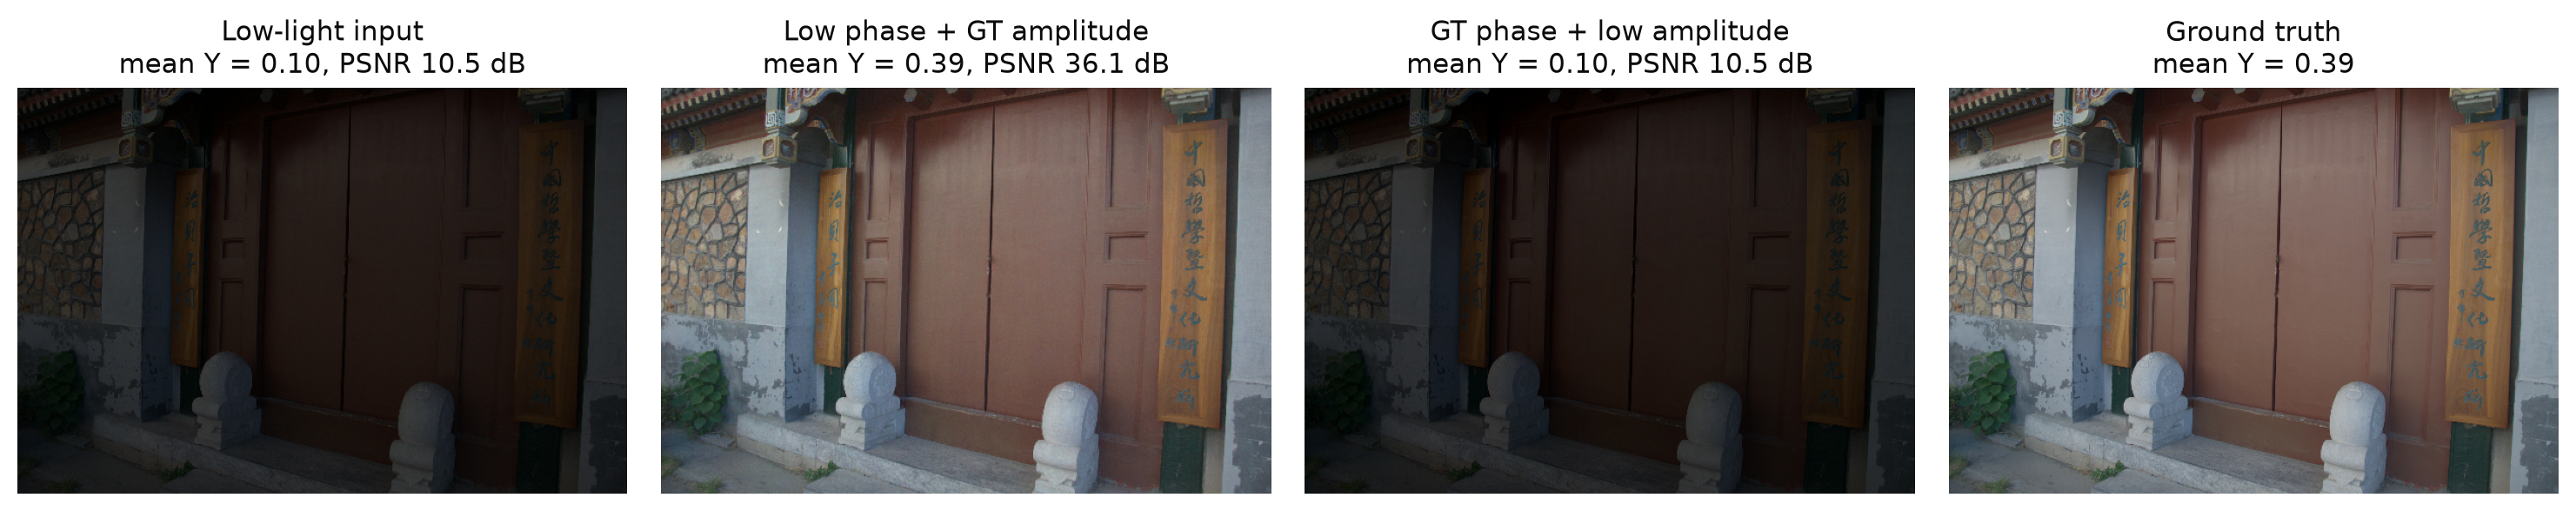
\includegraphics[width=\textwidth, height=0.36\textheight, keepaspectratio]{results/amplitude_swap.png}
    \end{center}
    \begin{columns}[t]
        \begin{column}{0.55\textwidth}
            \footnotesize
            \begin{itemize}
                \item Low-light \textbf{phase} + GT \textbf{amplitude} $\approx$ the GT image: mean PSNR \textbf{9.72 $\rightarrow$ 29.07\,dB} over 100 pairs.
                \item GT phase + low amplitude stays dark: brightness lives in the amplitude, structure in the phase.
            \end{itemize}
        \end{column}
        \begin{column}{0.43\textwidth}
            \footnotesize
            $\Rightarrow$ This explains the design: \textbf{FreMLP} edits only the amplitude, and letting it change the phase too \textbf{lowers PSNR by 0.60\,dB} (Table 6).
        \end{column}
    \end{columns}
\end{frame}

%---------------------------------------------------------
%	6. DEMO & IMPACT
%---------------------------------------------------------
\section{Demo}

\begin{frame}
    \frametitle{Product Demo: NightClear Web App}
    \framesubtitle{Web application built with Gradio}

    \begin{columns}[c]
        \begin{column}{0.62\textwidth}
            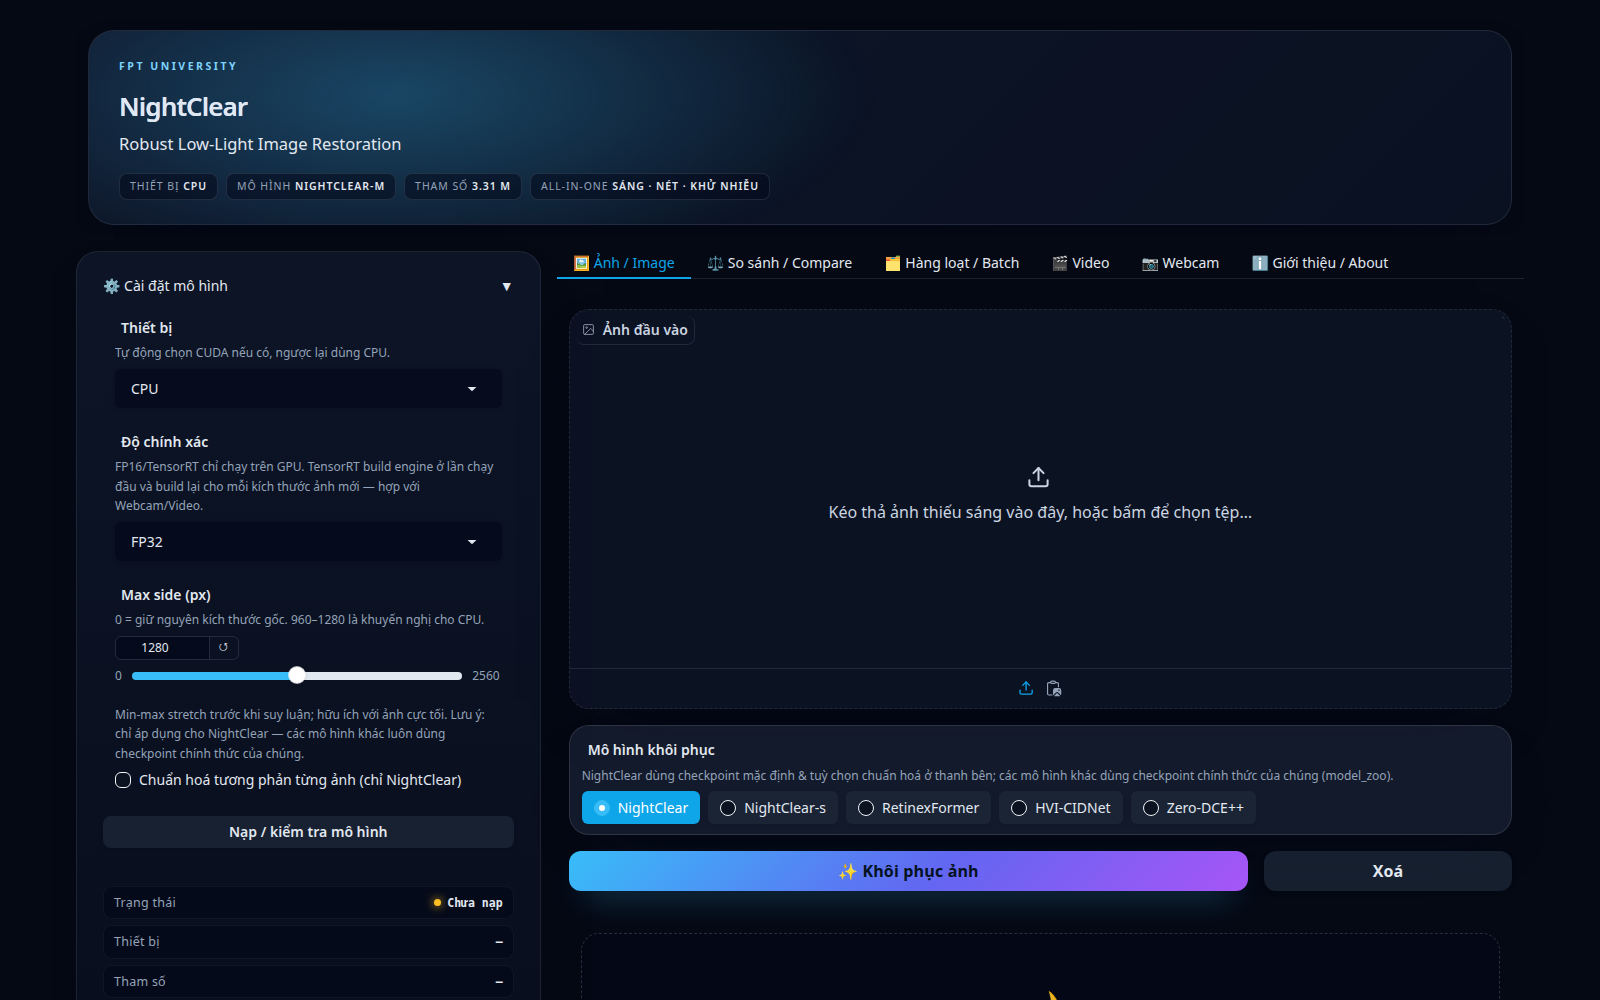
\includegraphics[width=\textwidth]{demo/ui.png}
        \end{column}
        \begin{column}{0.37\textwidth}
            \footnotesize
            \begin{itemize}
                \item \textbf{Tabs}: Image, Compare, Batch, Video, Webcam
                \item \textbf{5 models}: NightClear, NightClear-s, RetinexFormer, HVI-CIDNet, Zero-DCE++
                \item \textbf{Compare}: all models on one photo, ranked by speed
                \item \textbf{Precision}: FP32, FP16, TensorRT
                \item Runs on CPU or GPU, including free Google Colab
            \end{itemize}
        \end{column}
    \end{columns}
\end{frame}

% stat tile: big number + caption (defined outside the frame: frame bodies cannot hold #-parameters)
\newcommand{\stat}[2]{%
    \begin{beamercolorbox}[wd=\linewidth, ht=1.6cm, dp=0pt, center, rounded=true]{block body example}
        {\LARGE\bfseries\color{fptOrange} #1}\\[1mm]{\scriptsize #2}
    \end{beamercolorbox}}

\begin{frame}
    \frametitle{Practical Impact}

    \begin{columns}[t]
        \begin{column}{0.24\textwidth}\stat{+8.7 dB}{vs.\ best 2-model cascade}\end{column}
        \begin{column}{0.24\textwidth}\stat{5.3$\times$}{fewer MACs than LEDNet}\end{column}
        \begin{column}{0.24\textwidth}\stat{$-$55\%}{parameters vs.\ LEDNet}\end{column}
        \begin{column}{0.24\textwidth}\stat{3.31 M}{params, 13 MB, runs on CPU}\end{column}
    \end{columns}
    \vspace{2mm}
    \begin{columns}[t]
        \begin{column}{0.5\textwidth}
            \small
            \textbf{Value}
            \begin{itemize}
                \item One network instead of two to store, tune and run
                \item Fits laptops, edge and free cloud GPUs
                \item Handheld night shots without tripod or flash
            \end{itemize}
        \end{column}
        \begin{column}{0.5\textwidth}
            \small
            \textbf{Applications}
            \begin{itemize}
                \item Smartphone night mode
                \item Night surveillance / dash cams
                \item Pre-processing for detection in the dark (e.g.\ ExDark)
            \end{itemize}
        \end{column}
    \end{columns}
    {\tiny Numbers from paper Tables 1--2 (LOLBlur). The paper reports no runtime, so no time saving is claimed.}
\end{frame}

%---------------------------------------------------------
%	7. LIMITATIONS, CONCLUSION & Q&A
%---------------------------------------------------------
\section{Conclusion}

\begin{frame}
    \frametitle{Limitations \& Future Work}
    \begin{columns}[t]
        \begin{column}{0.5\textwidth}
            \footnotesize
            \textbf{Limitations}
            \begin{itemize}
                \item Depthwise convs: few MACs but not GPU-friendly, so speed gains are smaller than compute gains
                \item No runtime benchmark yet (only MACs / parameters)
                \item Not best on every metric (SSIM/LPIPS on LOLBlur, real photos)
                \item Real/synthetic gap in the data (EDA)
                \item Our app: TensorRT disabled for RetinexFormer / HVI-CIDNet (wrong outputs); NightClear-s weights not bundled
            \end{itemize}
        \end{column}
        \begin{column}{0.5\textwidth}
            \footnotesize
            \textbf{Future work}
            \begin{itemize}
                \item Measure latency on phone / edge GPUs; INT8 quantisation
                \item Video: temporal consistency between frames
                \item Collect real paired night data (e.g.\ with a tripod) to close the domain gap
                \item Train jointly with a detector for night-time object detection
            \end{itemize}
        \end{column}
    \end{columns}
\end{frame}

\begin{frame}
    \frametitle{Conclusion}
    \textbf{Key takeaways}
    \begin{enumerate}
        \item \textbf{One model, three problems}: NightClear brightens, denoises and deblurs at once and beats two-model pipelines by +8.7\,dB.
        \item \textbf{Efficient by design}: Fourier-amplitude encoder + dilated decoder give the best LOLBlur PSNR at 7.25 GMACs; our EDA and amplitude-swap test show why.
        \item \textbf{Deployable}: a web app with 5 models, video/webcam and FP16/TensorRT, runnable on CPU or a free GPU.
    \end{enumerate}
\end{frame}

%---------------------------------------------------------
%	REFERENCES (written by hand: biblatex is not installed on the build machine)
%---------------------------------------------------------
\begin{frame}[noframenumbering]
    \frametitle{References}
    \scriptsize
    \begin{enumerate}
        \item D. Feijoo, J. C. Benito, A. Garcia, M. V. Conde. \emph{DarkIR: Robust Low-Light Image Restoration}. CVPR 2025. arXiv:2412.13443.
        \item S. Zhou, C. Li, C. C. Loy. \emph{LEDNet: Joint Low-Light Enhancement and Deblurring in the Dark}. ECCV 2022.
        \item Y. Cai et al. \emph{Retinexformer: One-stage Retinex-based Transformer for Low-light Image Enhancement}. ICCV 2023.
        \item S. W. Zamir et al. \emph{Restormer: Efficient Transformer for High-Resolution Image Restoration}. CVPR 2022.
        \item L. Chen, X. Chu, X. Zhang, J. Sun. \emph{Simple Baselines for Image Restoration (NAFNet)}. ECCV 2022.
        \item Q. Yan et al. \emph{HVI: A New Color Space for Low-light Image Enhancement (HVI-CIDNet)}. CVPR 2025.
        \item C. Li, C. Guo, C. C. Loy. \emph{Learning to Enhance Low-Light Image via Zero-Reference Deep Curve Estimation (Zero-DCE++)}. TPAMI 2021.
        \item W. Yang et al. \emph{Sparse Gradient Regularized Deep Retinex Network for Robust Low-Light Image Enhancement (LOLv2)}. TIP 2021.
        \item J. Hai et al. \emph{R2RNet: Low-light Image Enhancement via Real-low to Real-normal Network (LSRW)}. JVCIR 2023.
    \end{enumerate}
\end{frame}

%---------------------------------------------------------
%	APPENDIX (backup slides, not counted)
%---------------------------------------------------------
\appendix

\begin{frame}[noframenumbering]
    \frametitle{Backup: Dataset Scale}
    \framesubtitle{Paired datasets, number of image pairs (README)}

    \begin{center}
        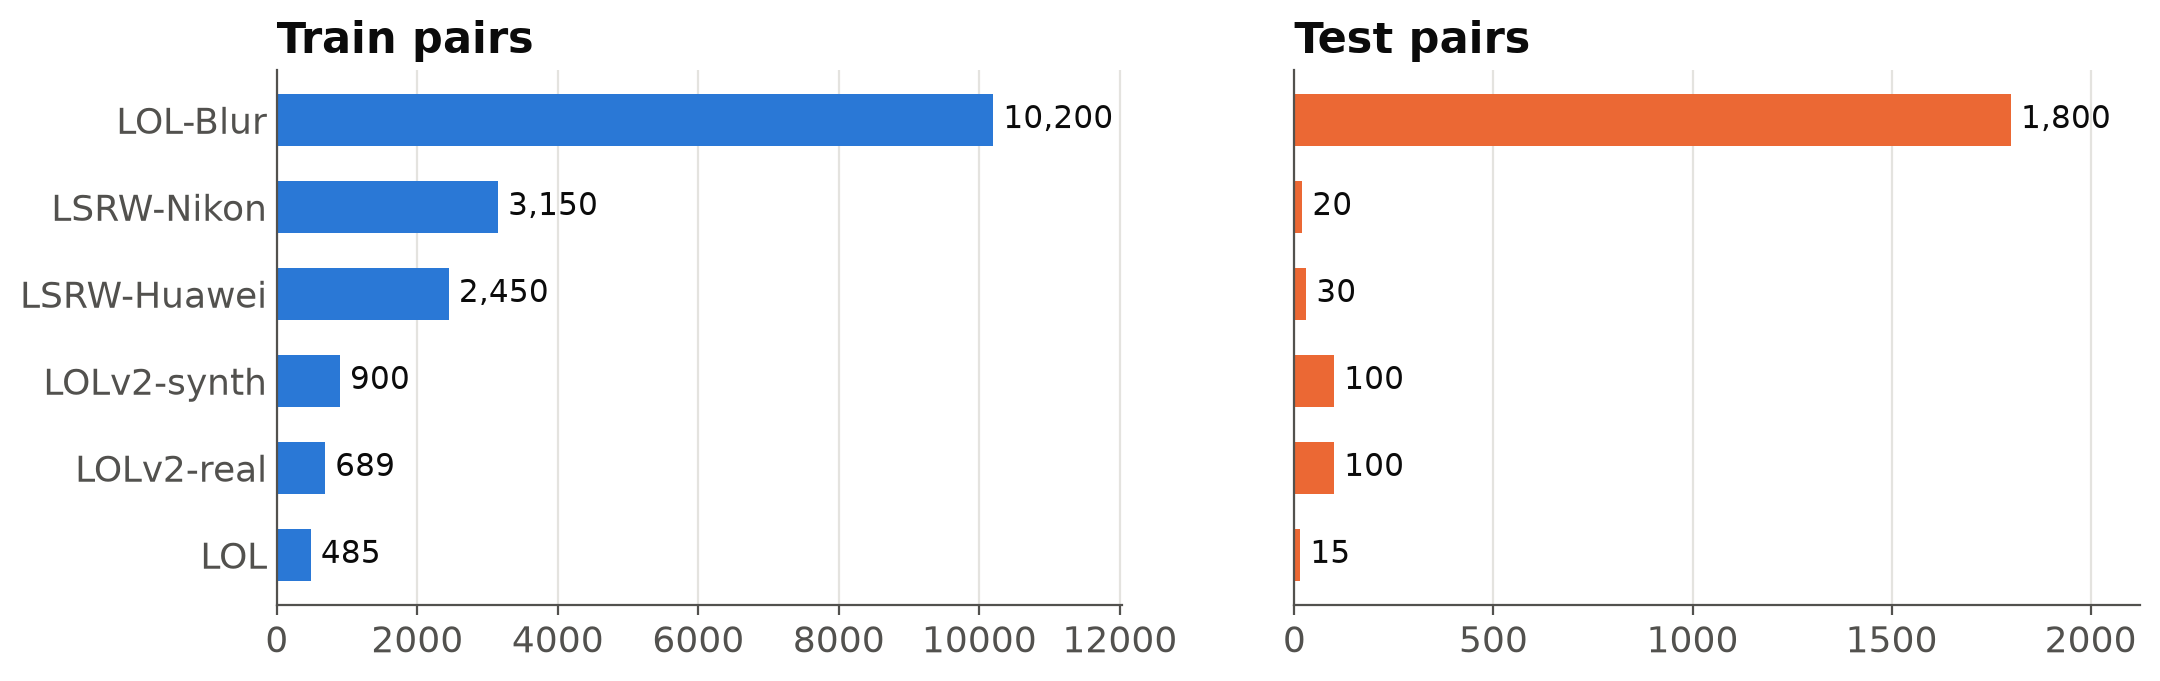
\includegraphics[width=0.95\textwidth]{eda/dataset_sizes.png}
    \end{center}
    {\footnotesize
    \begin{itemize}
        \item LOL-Blur alone has more training pairs than all other paired sets combined.
        \item Test sets are tiny for LOL (15) and LSRW (20--30): single-number scores there are noisy.
    \end{itemize}
    }
\end{frame}

\begin{frame}[noframenumbering]
    \frametitle{Backup: LOLv2 Samples}
    \framesubtitle{Low-light input (top) vs.\ normal-light ground truth (bottom), test split}

    \begin{center}
        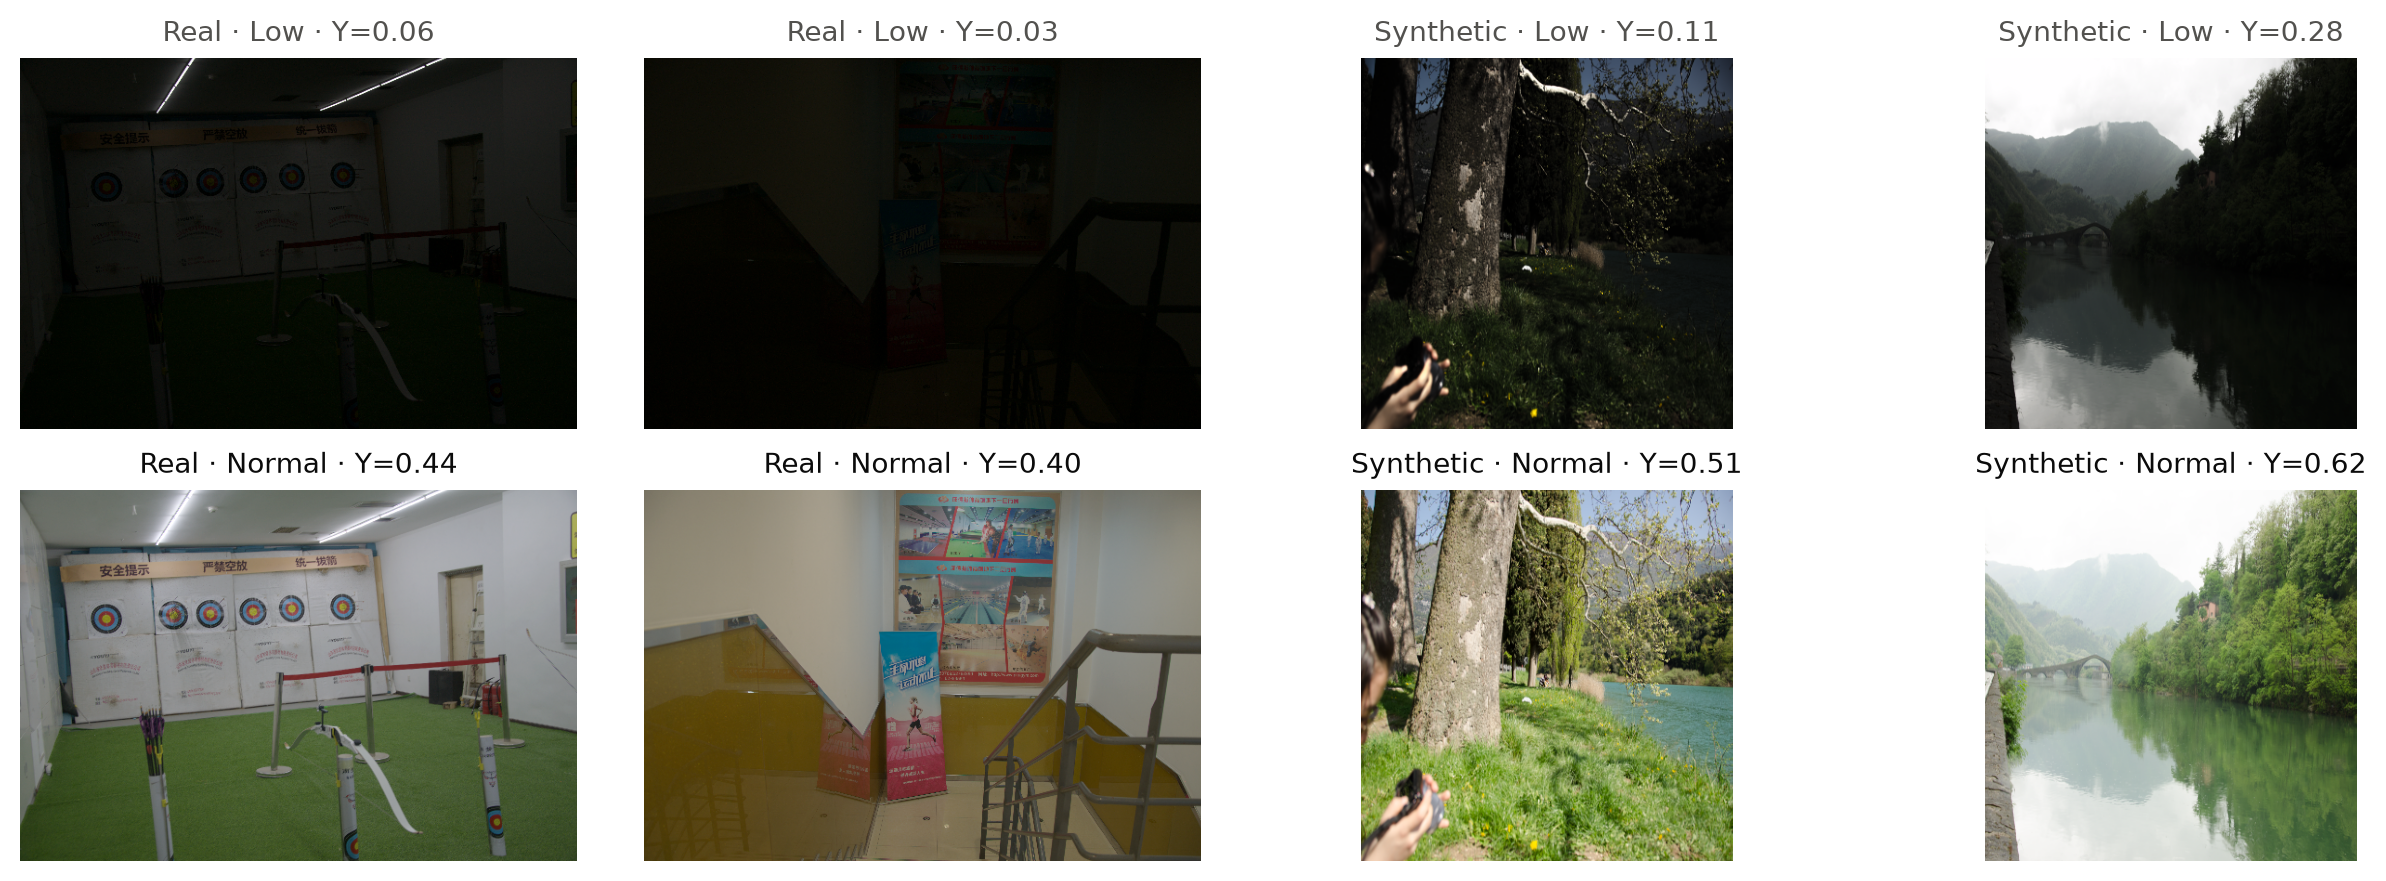
\includegraphics[width=\textwidth, height=0.6\textheight, keepaspectratio]{eda/samples.png}
    \end{center}
    {\footnotesize
    \begin{itemize}
        \item Real: 689 + 100 pairs, 600$\times$400. Synthetic: 900 + 100 pairs, 384$\times$384. All RGB, every low image has its ground truth.
    \end{itemize}
    }
\end{frame}

%---------------------------------------------------------
%	THANK YOU (final slide)
%---------------------------------------------------------
\begin{frame}
    \begin{center}
        
\includegraphics[height=1.3cm]{Logo_FPT_Education.png}\\[6mm]
        {\fontsize{40}{46}\selectfont\bfseries\color{fptBlue} Thank You!}\\[4mm]
        {\large\color{fptOrange} NightClear: Robust Low-Light Image Restoration}\\[6mm]
        {\small Mai Xuan Duc \quad$\cdot$\quad Phan Minh Nhat Truong \quad$\cdot$\quad Dang Thanh Tuan}\\[1mm]
        {\footnotesize Supervisor: Mr. Nguyen Trong Tai \quad$\cdot$\quad FPT University}
    \end{center}
\end{frame}


\end{document}
